% ---------------------------------------------------
% ----- Chapters of the template
% ----- for Bachelor-, Master thesis and class papers
% ---------------------------------------------------
%  Created by C. Müller-Birn on 2012-08-17, CC-BY-SA 3.0.
%  Freie Universität Berlin, Institute of Computer Science, Human Centered Computing. 
%
\chapter{Kapitel}
\label{chap:chapters} 

%\begin{itemize}
	%\item Abhängig vom Ziel der Arbeit und dem verwendeten Forschungsdesign
	% unterscheidet sich dieser Hauptteil der Arbeit erheblich.
	%\item Eine sehr allgemeine Struktur ist die folgende:
	%\begin{itemize}
		%\item Hintergrund der Arbeit (Theoretische Einordnung der Arbeit)
		\section{Hintergrund der Arbeit}
		\subsection{Mapping Methoden}
		Der grundlegende Prozess für die Bestimmung möglicher Matches von Eigenschaften
		sieht wie in Abbildung \ref{fig1} gezeigt aus. Das zentrale Element dabei ist
		der oder die Matcher. \cite{Hoo14}
		
		\begin{figure}[ht]
		\centering
		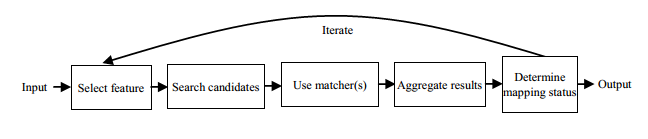
\includegraphics[width=1.0\textwidth]{pics/simple-high-level-view-of-a-mapping-process.png}
		\caption{Eine einfache Übersicht des Mapping Prozesses \cite{Hoo14}}
		\label{fig1}
		\end{figure}
		
		Im ersten Schritt wird ein Element (\textit{feature}), wie ein Label für
		Entitäten oder Instanzen von Attributen, aus einer der zu matchenden Ontologien ausgewählt,
		anschließend werden in der anderen Ontologie nach möglichen, passenden
		Elementen (sogenannte \textit{candidates}) gesucht. Mithilfe der Matcher werden
		die beiden Eigenschaften dann verbunden, sofern der oder die Matcher Übereinstimmungen vermuten. Die Ergebnisse werden dann zusammengefasst und zum Schluss entweder in einer neuen Iteration berücksichtigt oder ausgegeben. \cite{Hoo14}\\
		Neben der direkten Verbindung kann man die Eigenschaften aus den Ontologien, die
		gematched werden sollen, über sogenannte \textit{Anker} (Anchors) mit einer
		weiteren Ontologie verbunden, deren Zweck es ist, als „Meta-Ontologie“ eine gemeinsame Schnittstelle zu bilden. Anker sind Entitäten, die als gleichartig zu Entitäten der anderen Ontologien definiert werden. \cite{Hoo14}
		
		\subsection{Kategorien von Matchern}
		Um Ontologien zu matchen gibt es verschiedene Möglichkeiten. Diese können einzeln, aber auch kombiniert auf verschiedene Weise angewendet werden. Eine Möglichkeit ist es, mehrere Matcher sequentiell anzuwenden, um die Ergebnisse immer mehr zu verfeinern und zu verbessern. Eine andere Variante ist es, mehr als eine Matching Methode parallel anzuwenden und dann die Ergebnisse zusammenzufügen. Diese beiden Aggregationsverfahren kann man auch kombinieren. \cite{Hoo14}
		
		\subsection{Terminologisches Mapping}
		Um Elemente von Ontologien zu matchen, kann man deren Benennung durch Tokenisierung in ein gemeinsames Format überführen und dann mithilfe von Gewichtung und Gleichheit in Relation setzen.
		\begin{itemize}
			\item Stringbasiert: Bei dieser Methode wird die Struktur von Strings als
			Zeichenketten betrachtet. Konkret werden Techniken angewendet, die Ähnlichkeit von Strings und deren Teilen bestimmen. Bekannte Methoden aus diesem Bereich sind z.B. Normalisierung und Editierdistanz. \cite{Euz07}  Beispielsweise beträgt der Abstand der Elemente „author“ und „hasauthor“ 3, nämlich den Zusatz „has“, sofern der Algorithmus erkennt, dass der hintere Teil gleich ist.
			\item  Sprache basiert: Hierbei werden Wörter als Texte betrachtet, d.h. die
			Reihenfolge der Wörter in einer Sequenz wird einbezogen, ebenso die Bedeutung dieser Wörter. Zur Analyse werden verschiedene Techniken angewandt, um das Grundwort zu ermitteln. Dieses dient dann dazu, Ähnlichkeiten zwischen den Wörtern zu finden. \cite{Euz07}  Zum Beispiel, wenn man in einer Ontologie das Element „walk“ und in einer anderen „walking“ hat, kann man „walking“ auf „walk“ reduzieren (z.B. durch Stemming) und dadurch Matches finden.
			\item Linguistische Analyse: Durch das Einbeziehen von externen
			linguistischen Quellen, wie z.B. Wiktionary , werden Strings interpretiert.
			Beim bedeutungsbasierten Ansatz werden über \textit{Hyponyme} (begriffliche
			Unterordnung), \textit{Hyperonyme} (Ober-/Überbegriff), \textit{Synonyme}
			(gleiche Bedeutung) und \textit{Antonyme} (gegensätzliche Bedeutung) die
			Bedeutung der Wörter festgestellt. Beim sprachbasierten Ansatz hingegen, wird der Abstand zu anderen Wörtern in Sätzen analysiert. \cite{Euz07} Zum Beispiel kann man „creator“ als Oberbegriff von „author“ und „illustrator“ auffassen.
		\end{itemize}
		
		\subsection{Strukturelles Mapping}
		Eine zweite Möglichkeit für das Matching von Ontologien ist das Betrachten der Strukturen innerhalb der Ontologien. Dabei werden die Eigenschaften und die Beziehung der Entitäten untereinander untersucht.
		\begin{itemize}
			\item Taxonomisches Mapping: Dabei werden zwei Techniken verwendet,
			\textit{super-} oder  \textit{subclass rule} und \textit{bounded-paths}. Die
			\textit{super class rule} unterstellt, dass eine Ähnlichkeit zwischen zwei
			Konzepten besteht, wenn diese ein Elternkonzept teilen. \cite{Euz07}  Beispielsweise kann man annehmen, dass wenn zwei Ontologien ein gleiches oder ähnliches Konzept haben, um Bücher zu beschreiben, dass die darunterliegenden Konzepte für die Beschreibung für „creator“ und „author“ ebenfalls ähnlich bzw. gleich sind. Bei bounded-paths werden Pfade verglichen, um ähnliche Konzepte zu identifizieren. Bei diesen Pfaden handelt es sich um Verbindungen zwischen Klassen. Die Art und Weise der Verbindungen wird durch eine hierarchische Struktur definiert. \cite{Euz07} Wenn das Attribut „book“ in zwei verschiedenen Ontologien einmal mit „hasAuthor“ und einmal mit „hasWritten“ zu den beiden äquivalenten Elementen „creator“ bzw. „author“ verbunden ist, dann bieten sich diese beiden für eine Betrachtung bezüglich eines Matches an.
			\item Baumbasiertes Mapping: Hierbei spielt Ähnlichkeit eine Rolle. Es wird
			angenommen, dass sich Knoten ähneln, die benachbart sind, und dass dies auch für verschiedene Ontologien gilt. Also wenn ein Knoten mit einem anderen benachbart ist und mit einem Knoten aus einer anderen Ontologie verbunden ist, dann ähneln sich die benachbarten Knoten mit den beiden verbundenen. Wenn beispielsweise in einer Ontologie das Element „book“ über „author“ mit „human“ verbunden ist und in einer zweiten Ontologie „volume“ über „author“ mit „writer“, wobei festgelegt wurde, dass sowohl „book“ und „volume“, als auch die beiden „author“ Elemente äquivalent sind, besteht Grund zur Annahme, dass „human“ und „writer“ ebenfalls ähnlich sind. \cite{Euz07} 
		\end{itemize}
		
		\subsection{Recommender Systems}
		Als Recommender Systeme werden Software und Techniken bezeichnet, die dazu
		dienen, ihren Anwendern sinnvolle Vorschläge bezüglich Entscheidungen zu machen. Meist sind diese Systeme darauf hin ausgerichtet, unerfahrene oder nicht sachkundige Nutzer zu unterstützen. \cite{Fra10}  Bekannt sind den meisten Menschen solche System überwiegend aus den Bereichen des eCommerce, wo sie genutzt werden, um Kunden oder Besuchern Produkte vorzuschlagen, die diese interessieren könnten.\\
		In ihrer einfachsten Form, werden möglich Vorschläge in einer Liste gesammelt und dann entsprechend der Präferenzen des Nutzers und (Rand-)Bedingungen geordnet. Beide ergeben sich direkt, z.B. beim Ansehen eines Produkts in einem Webshop, oder indirekt, z.B. über die Empfehlung eines Films des gleichen Regisseurs. \cite{Fra10} 
		
		\subsection{Information Visualization}
		Bei der Information Visualization geht es im Kern darum, Daten grafisch
		darzustellen. Dadurch ist es möglich, Daten anzuzeigen, um den
		Nutzer bzw. Betrachter nicht das Interesse verlieren zu lassen. Weiterhin ermöglichen eine gute Aufbereitung der Daten und ein
		gutes User Iterface (UI) ein leichteres Navigieren innerhalb dieser Daten und deren Verknüpfung.\\
		Dafür gibt es eine Reihe an Techniken, um dies zu bewerkstelligen. Die
		Visualisierung von Informationen ist eng verknüpft mit der \textit{visuellen
		Datenexploration} (visual data exploration).
		Bei der visuellen Datenexploration werden Daten visualisiert, um es Menschen zu
		ermöglichen, diese Daten zu durchdringen, Schlüsse aus ihnen zu ziehen und direkt mit den Daten zu interagieren. \cite{Kei02}\\ Die manuelle Exploration von Daten kann zum Generieren von Hypothesen auf Basis von Daten genutzt werden, zusätzlich zur Anwendung von automatisierten Techniken aus der Statistik oder Machine Learning. Da diese beiden Arten von Techniken nicht immer anwendbar sind, kann man trotzdem gute Ergebnisse bei der Auswertung erzielen. Insbesondere wenn es  sich um stark inhomogene oder stark verrauschte Daten handelt. Zusätzlich kann man Datenexploration oft auch dann durchführen, ohne tiefgreifendes Verständnis von komplexen  mathematischen oder statistischen Algorithmen oder Parametern zu haben. \cite{Kei02} 
		
		\section{Vorhandene Software}
		Da es bereits Software für den Umgang mit Ontologien und das Matchen derselben gibt, wird sie an dieser Stelle betrachtet. Zum einen, um das Rad in diesem Bereich nicht neu und möglicherweise schlechter zu erfinden, sondern zu erweitern und/oder andere Aspekte zu behandeln. Und zum anderen soll von bestehenden Tools gelernt werden. Da die Auswahl an möglichen Tools groß ist \cite{Ber14} , können nicht alle in diesem Rahmen ausführlich vorgestellt werden. Daher erfolgt hier nur eine Auswahl. Reine Frameworks wurden bei der Bewertung nicht beachtet, da diese für die Zielgruppe nicht technischer Experten nicht geeignet sind, sondern für Entwickler von entsprechenden Tools.
		
		\subsection{AgreementMakerLight}
		\textit{AgreementMakerLight} ist ein automatisiertes Ontologie Matching System,
		das eine Weiterentwicklung der Software AgreementMaker ist und seit Anfang 2013 entwickelt wird. Der AgreementMakerLight ist Open Source, wird unter der Apache Lizenz Version 2.0 veröffentlicht und kann daher frei weiterentwickelt und verwendet werden. Es ist ein erweiterbares Framework und will Probleme bei umfangreichen Ontologie Matchings durch Effizienz angehen. Hauptsächlich finden Techniken Anwendung, die auf Elementebene arbeiten und durch domänspezifisches Wissen ergänzt werden.
		Der AgreementMakerLight wird als vorbereitetes Projekt für die Integrated
		Development Environment (IDE) Eclipse und als ausführbares Java-Archiv (jar) angeboten. Beides trifft die gewählte Zielgruppe aber nicht. Als Projekt ist es eher für Entwickler oder zumindest mit Softwareentwicklung vertrauten Personen gerichtet. Um eine jar-Datei auszuführen, ist eine Installation von Java nötig, was dem Gedanken des im Rahmen dieser Arbeit zu erstellenden Tools widerspricht, unkompliziert und sofort benutzbar zu sein.
		
		\subsection{PARIS}
		\textit{PARIS}, kurz für Probabilistic Alignment of Relations, Instances, and
		Schema, ist ein System, um Ontologien im RDF Format zu matchen. Dabei werden Verbindungen
		auf Instanz- und Klassenebene gesucht und wirken sich aufeinander aus. Matchings wird eine Wahrscheinlichkeit zugerechnet, um ohne das Festlegen von Parametern zu arbeiten. In Tests mit großen Ontologien erzielt PARIS eine Trefferquote von etwa 90\%. PARIS steht unter einer Creative Commons Lizenz , die eine kommerzielle Nutzung untersagt und eine Namensnennung der Ersteller vorschreibt. Ansonsten ist die Erweiterung und Nutzung aber frei\\
		PARIS wird neben dem reinen Quellcode als jar-Datei ausgeliefert. Wie beim AgreementMakerLight ist dies für die Zielgruppe kein idealer Anwendungsfall. Weiterhin wird PARIS über die Kommandozeile gestartet, im Gegensatz zu z.B. AgreementMakerLight, was eine zusätzliche Hürde darstellt.
		
		\subsection{COMA 3.0}
		\textit{COMA 3.0} ist Matching Tool für Schemata und Ontologien und wurde am
		Institut für Informatik an der Universität Leipzig entwickelt. Es gibt sowohl eine klassische Software- als auch eine Webversion. Beide wurden in Java entwickelt. Die Webversion wird als Java Applet angeboten. Die Vorgänger von COMA 3.0 hießen COMA und COMA++ und es ist eine Weiterentwickelung von diesen. Dafür wurden das Management des Workflows verbessert und Features hinzugefügt, darunter Ontologie Matching.
		Da die im Rahmen dieser Mastarbeit entwickelte Software als Webapplikation entwickelt werden soll, wird wegen der Ähnlichkeit nur das Java Applet betrachtet. Als Java Applets wird Java Software in Java Bytecode bezeichnet, die über einen Webbrowser ausgeführt werden kann.  Dafür werden in Browsern Plug-Ins benötigt, die in der Regel aber nicht vorinstalliert sind. Auch gab es immer wieder Probleme mit Sicherheitslücken und „das Java-Plug-in war als einer der größten Türöffner für Sicherheitsangriffe bekannt und wurde in Untersuchungen immer wieder als Risiko Nummer eins auf den PCs dieser Welt bezeichnet“.  Zu Beginn des Jahres 2016 wurde von Oracle, dem Hersteller von Java, verkündet, dass diese Technologie nicht mehr weiterentwickelt wird.  Weiterhin ist die Portabilität über Betriebssysteme nicht unproblematisch, da Browser auf mobilen Geräten, die Plug-Ins fast ausnahmslos nicht unterstützen.  Das sind alles Gründe, die gegen einen Einsatz im Benutzerkreis sprechen, der im Rahmen dieser Mastarbeit angesprochen werden soll.
		
		\subsection{LODE}
		\textit{LODE} (Linked Open Data Enhancer) ist ein webbasiertes Tool, um
		Ontologien zu erkunden, zu matchen und zu erweitern. Es ist Open Source  und wird innerhalb des Play Frameworks   verwendet. Entwickelt wurde es in der Kooperation der Universitäten Mannheim, Washington und Indiana.
		
		\subsection{HerTUDA}
		\textit{HerTUDA} ist ein Ontologie Matching Tool der Knowledge Engineering
		Arbeitsgruppe des Fachbereichs Informatik an der Technischen Universität Darmstadt. Es ist auf schnelles und einfaches Arbeiten ausgelegt und arbeitet mit syntaktischen Vergleichen von Strings und Herausfiltern irrelevanter Matches.
		 		%\item Hier sollte enthalten sein, welche Anwendungen in diesem Bereich
		 		% bereits existieren und warum bei diesen ein Defizit besteht.
				%\item Falls genutzt, sollten hier die entsprechenden Algorithmen erläutert
				% werden.
				%\item Es sollten die Ziele der Anwendungsentwicklung, d.h. die
				% Anforderungen herausgearbeitet werden. Dabei sollte die bestehende Literatur geeignet integriert werden.
		 	%\end{itemize}
		%\item Umsetzung (Praktischer Anteil der Arbeit)
			%\begin{itemize}
				%\item Zunächst sollte die Softwarearchitektur und die genutzten
				% Anwendungen, APIs etc. erläutert werden. Ebenfalls gehört dazu das Datenbankschema.
				%\item Es sollten die zentralen Elemente der Software (abhängig von der
				% Aufgabenstellung) beschrieben werden, wie implementierte Algorithmen oder das Oberflächendesign.
				%\item Zentraler Quellcode sollte entsprechend aufgelistet werden:
				%\lstset{language=Java,basicstyle=\footnotesize,numbers=left,showstringspaces=false,frame=single}
				%\begin{lstlisting}
				%public class Main {
				%	public static void main(String[] args) {
				%		System.out.println("Hello World!");
				%	}
				%}
				%\end{lstlisting} 
				%\item Klassendiagramm für Backend
				%\item Dr Quellcode zentraler Implementierungen  können als Auszug in den Anhang. Im Text kann dann darauf verwiesen werden.
			%\end{itemize}
		\section{Umsetzung}
		Die im Rahmen dieser Masterarbeit entwickelte Software besteht aus einem
		modularen Kern und ist über verschiedene Technologien ansprechbar. Aktuell
		sind die Matcher als App
		für Django\footnote{\url{https://www.djangoproject.com/}} verfügbar, können
		aber auch direkt in Python Skripten benutzt werden.\\
		Der Kernteil besteht aus mehreren Modulen, für die weitere Module
		implementiert werden können, um verschiedene Arten von Daten eingelesen
		werden können, z.B.
		Formate wie OWL/XML, Query Languages wie SPARQL oder REST-Schnittstellen.
		Zusätzlich können unterschiedliche Arten und Implementierungen von Matchern
		verwendet werden. Um dies zu realisieren, gibt es eine Klasse, um Ontologien,
		deren Elemente und Eigenschaften abzubilden, namens \textit{ontology}.
		Die Elemente dieser Instanzen bestehen wiederum aus Instanzen der Klasse
		\textit{onto element}. Dort enthalten sind alle Informationen, die das Element
		beschreiben. Diese beiden Klassen dienen als Schnittstellen, um innerhalb der
		Software mit Ontologien und deren Elementen zu interagieren.
		
		\subsection{Architektur}
		Sowohl die Kernmodule als auch die einzelnen, konkreten Ausführungen dieser
		Module sind entlang eines Prozesses organisiert, wie in Abbildung \ref{fig2}
		gezeigt.
		\begin{figure}[ht]
		\centering
		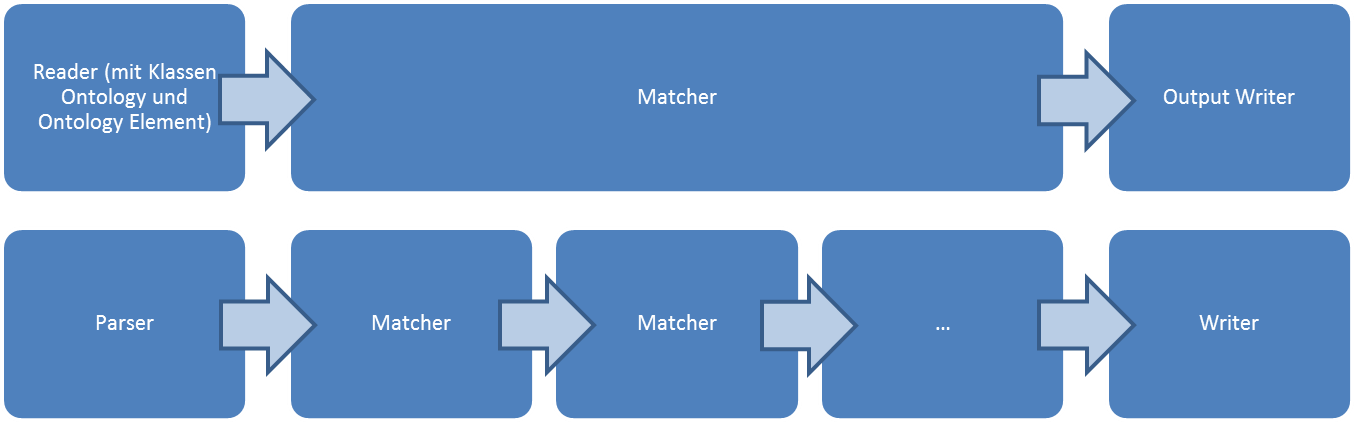
\includegraphics[width=1.0\textwidth]{pics/Module-overview.png}
		\caption{Prozessablauf der Module}
		\label{fig2}
		\end{figure}
		An erster Stelle stehen der oder die Parser, die die Ontologien einlesen und
		die Daten in Instanzen der Klasse \textit{ontology} einpflegen. Hierbei können
		auch Daten aus unterschiedlichen Quellen und beliebigen Formaten verwendet
		werden, sofern ein \textit{Reader} implementiert wurde. Im Rahmen dieser
		Masterarbeit wurden bereits einige implementiert, die einige gängige
		Möglichkeiten abdecken. Durch die Modularität können aber problemlos weitere
		hinzugefügt werden.\\
		Dann werden die Ontologien an verschiedene Matcher übergeben. Dabei werden
		die Ergebnisse von einem Matcher zum nächsten weitergegeben, so ist es zum
		einen möglich, diese Ergebnisse zu akkumulieren und zum
		anderen, weitergehende Analysen z.B. der Struktur oder Hierarchie vorzunehmen.
		Die Gesamtergebnisse werden dann an einen \textit{Output Writer} übergeben, um
		sie dann weiter bearbeiten zu können.\\
		
		
		\subsubsection{Anwendungsfall 1: Django App}
		Wenn die Module der Matching Software als Teil einer Django App genutzt
		werden, werden über ein
		Skript\footnote{SimpleOntologyMatcher/OntologyMatcher/settings.py} von Django
		mögliche Ontologien und Matcher gesammelt.
		
		\begin{figure}[ht]
		\centering
		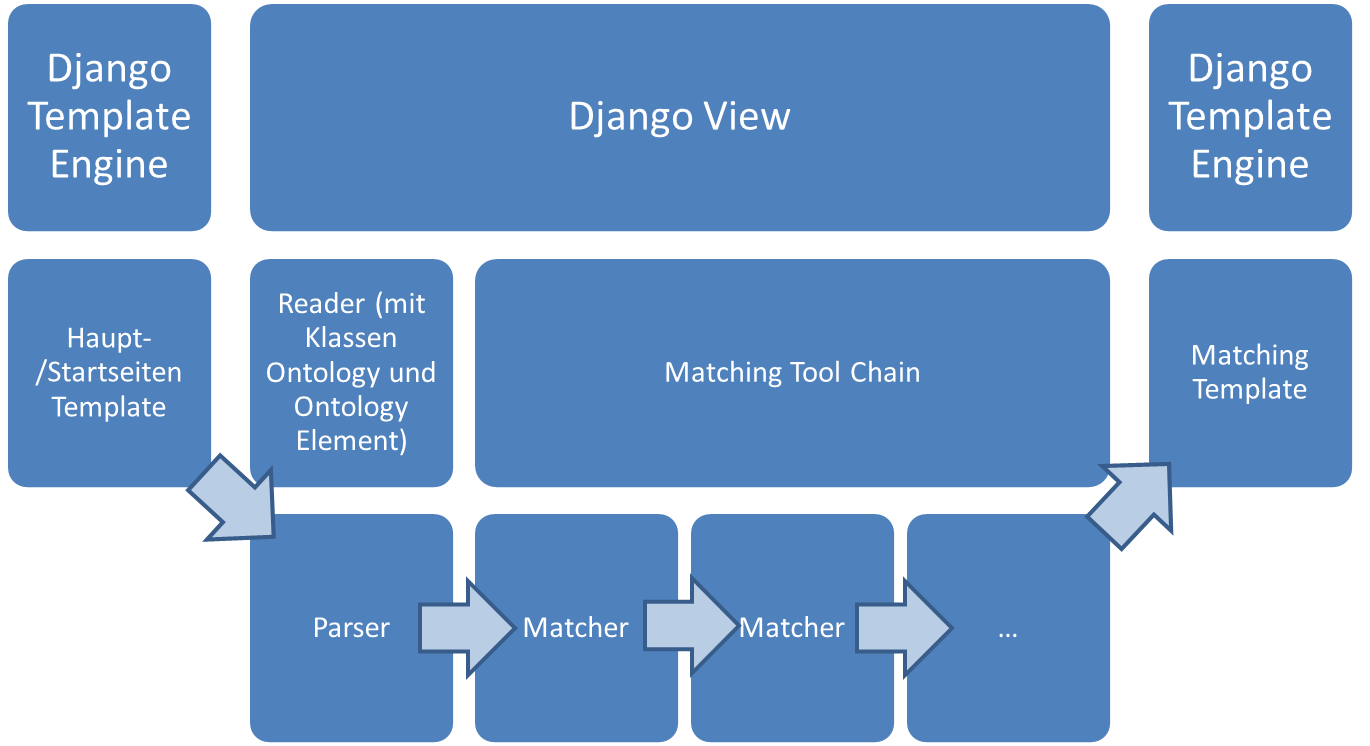
\includegraphics[width=1.0\textwidth]{pics/Module-overview1.png}
		\caption{Module Django App}
		\label{fig6}
		\end{figure}
		Dabei können, wie erwähnt, verschiedene Quellen verwendet werden. Für
		Ontologien sind lokale und auf externen Servern gespeicherte Dateien und in Datenbank
		eingepflegte Daten möglich. Bei Matchern werden nur lokal vorhandene Python
		Module berücksichtigt. Die gefundenen Ontologien und Matcher werden dann in
		ein HTML Template eingebetet, dass mit der textit{Django Template Engine} erstellt wird. Dabei wird auch die Quelle gespeichert, also der Dateiname mit Pfad oder
		die URL.\\
		Über die dann erstellte Seite können Ontologien ausgewählt werden, die
		analyisert werden sollen, und Matcher, mit denen dies durchgeführt wird.\\
		Das Design ist möglichst simpel gewählt, wie in \ref{fig3} gezeigt. Dadurch
		wird die Bedienung und gleichzeitig die Komplexität zu verringert, da die
		Optionen und Bedienung limitiert sind. Die GUI ist auf das Nötigste
		reduziert und nicht überfrachtet. Ein einfaches User Interface hilft auch bei
		der Akzeptanz, da der Einstieg ohne Vorkenntnisse auch für Fachfremde Personen
		erleichtert wird.
		
		\begin{figure}[ht]
		\centering
		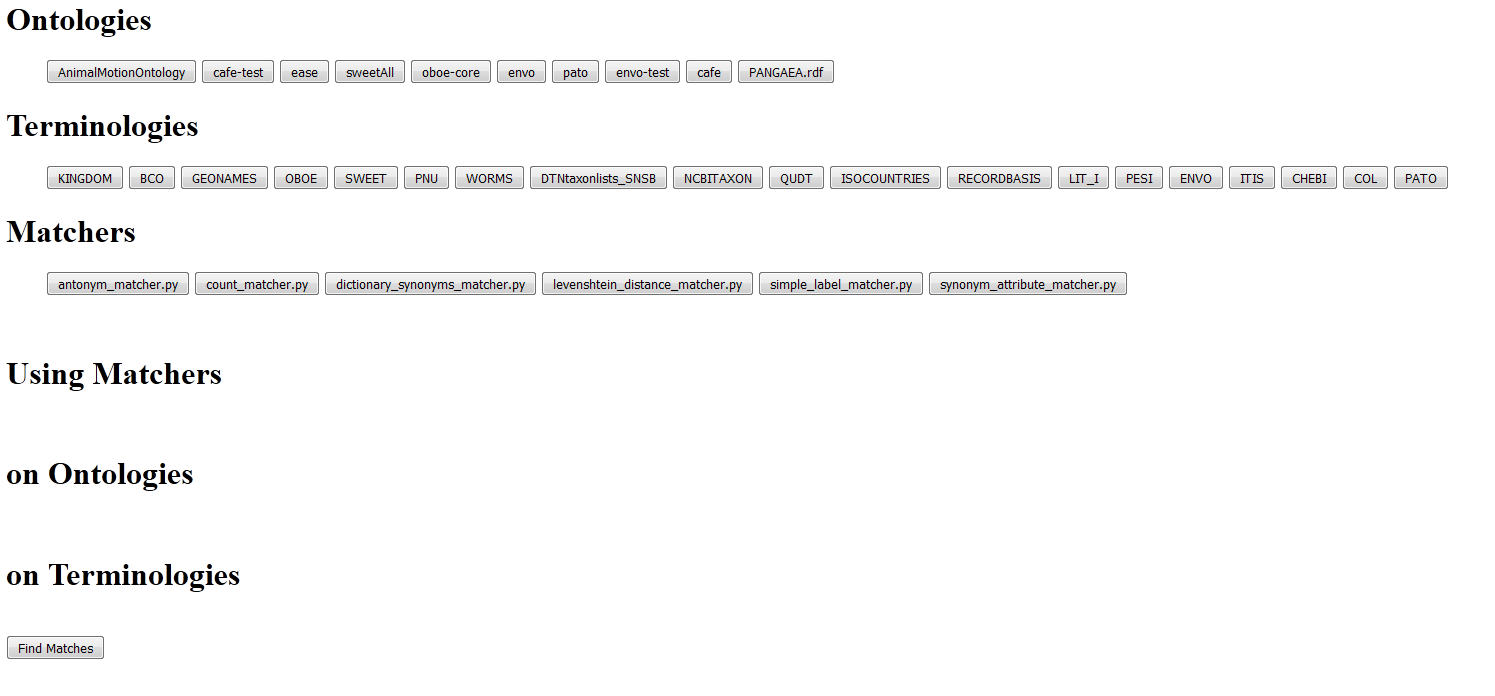
\includegraphics[width=1.0\textwidth]{pics/TemplateMatchingStartPage.png}
		\caption{Startseite Django App 1}
		\label{fig3}
		\end{figure}
		Wenn sowohl Ontologien bzw. Terminologien als auch mindestens ein Matcher
		gewählt wurden, wird der Matching Prozess, wie in \ref{fig4} gezeigt,
		gestartet.
		
		\begin{figure}[ht]
		\centering
		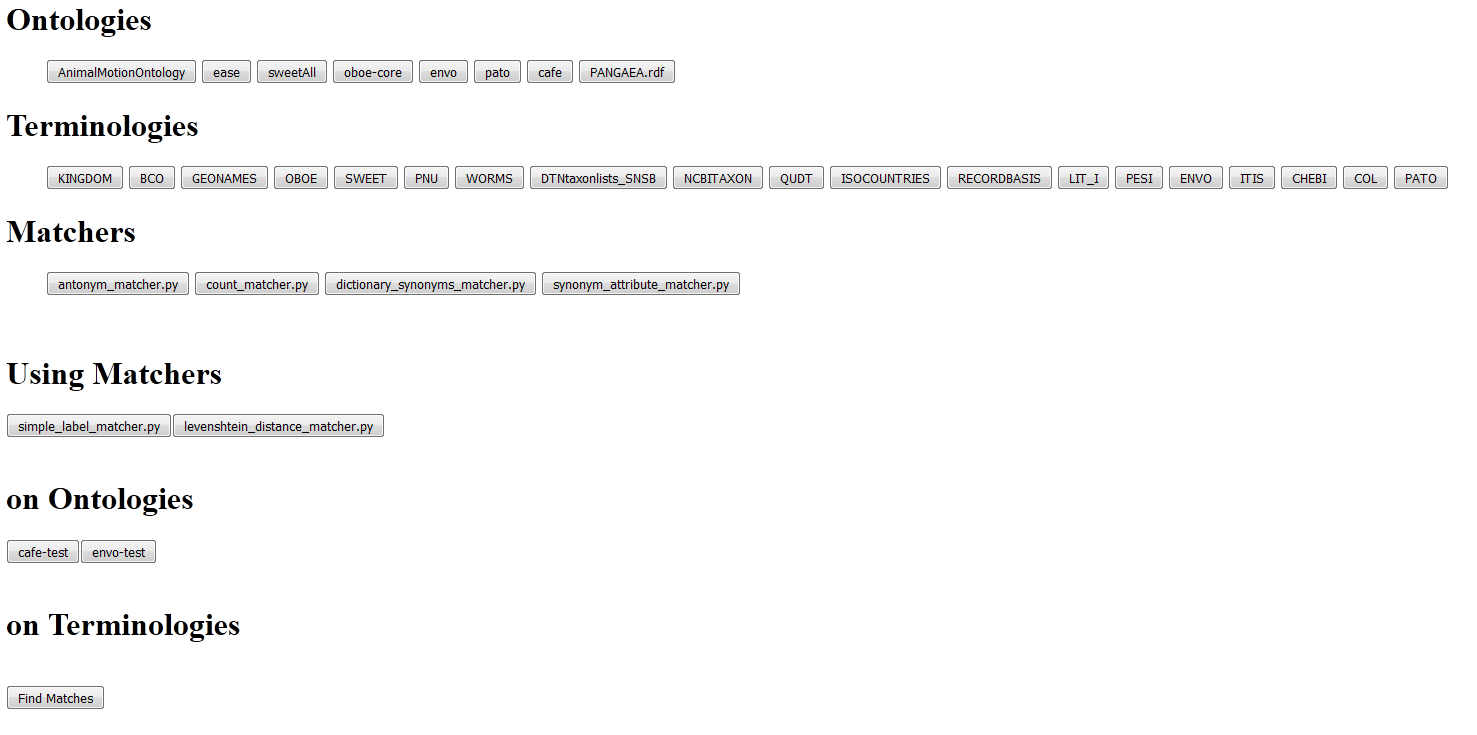
\includegraphics[width=1.0\textwidth]{pics/TemplateMatchingStartPage1.png}
		\caption{Startseite Django App 2}
		\label{fig4}
		\end{figure}
		Anschließend werden die ausgewählten Ontologien mit entsprechenden
		\textit{Readern} geparst. Die Reader werden ermittelt, indem überprüft wird,
		ob es sich bei der gespeicherten Quelle um eine URL oder eine
		existierende Datei handelt. Dies wird über das \textit{View} von Django
		erledigt und dann an das \textit{Reader} Modul weitergeleitet. Dieses bindet
		die passenden Module ein, startet das Parsen und liefert die Ergebnisse
		zurück. Die Ergebnisse bestehen aus Instanzen des Moduls \textit{onto} in
		einer Liste.\\
		Mit den übergebenen Matchern wird eine \textit{Matching Tool Chain} im
		gleichnamigen Modul erstellt, welche die Matcher in der angegebenen
		Reihenfolge ausführt. Die Ergebnisse jedes Matching Vorgangs werden von einem
		Matcher an den nächsten in Form des Python Datentyps \textit{Dictionary}
		weitergegeben. Dadurch ist es möglich, auf vorherige Ergebnisse zuzugreifen,
		um z.B. die Struktur zu analysieren. Die eigenen Ergebnisse eines Matchers
		werden einfach zum Dictionary hinzugefügt.\\
		Wenn alle Matcher durchlaufen wurden, wird das letztendliche Ergebnis in einem
		anderen Template der Django Template Engine verarbeitet und angezeigt,
		wie in \ref{fig5} exemplarisch dargestellt.
				
		\begin{figure}[ht]
		\centering
		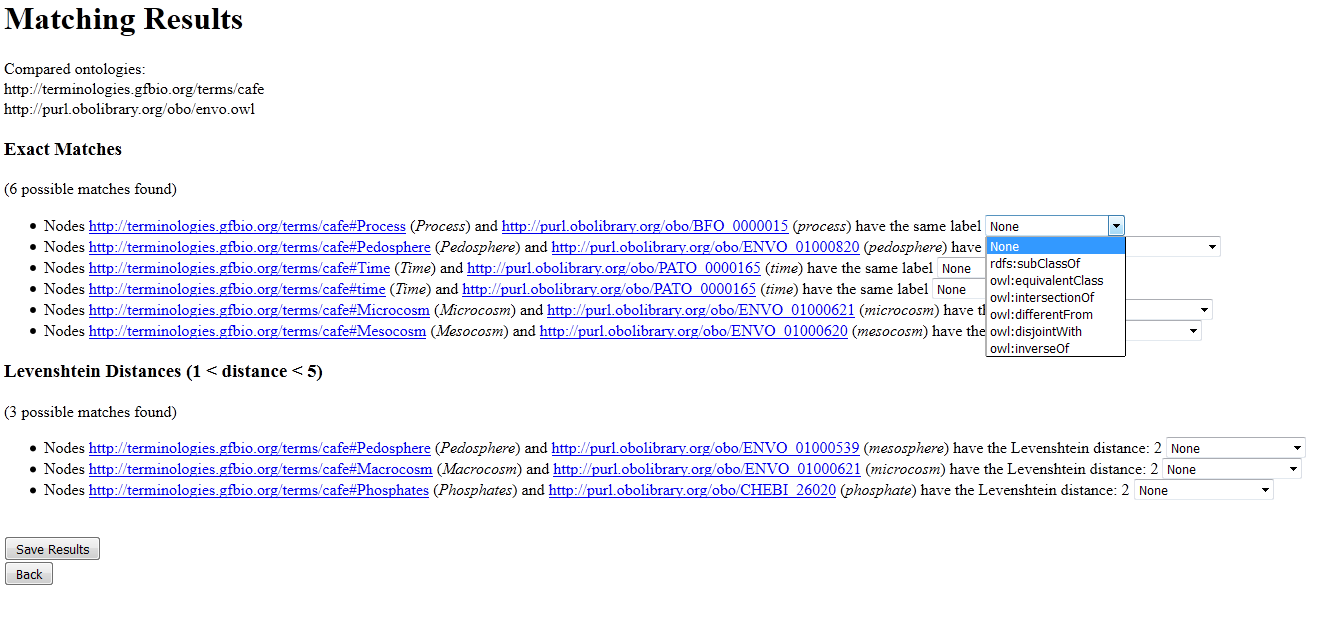
\includegraphics[width=1.0\textwidth]{pics/TemplateMatchingResultPage.png}
		\caption{Django App Resultatseite}
		\label{fig5}
		\end{figure}
		Auf dieser Seite kann dann gewählt werden, ob zwei Elemente eine Verbindung
		haben und welche dies ist. Wenn allen Paaren von Elementen eine Art von
		Verbindung oder eben keine zugeordnet wurde, ist es möglich, das Ergebnis in
		eine Datei im XML Format zu exportieren.
		
		\subsubsection{Anwendungsfall 2: Python Skript}
		Neben der Möglichkeit den Simple Ontology Matcher als Django App zu verwenden,
		können die einzelnen Module auch wie üblich als normale Python Module
		importiert und aufgerufen werden. Dabei ist es möglich, die Module der
		Zwischenschicht\footnote{matcher.py und reader.py} zu verwenden oder
		auszulassen, da diese nur das dynamische Einbinden übernehmen.
		
		\subsection{Implementierte Matcher}
		Im Rahmen dieser Masterarbeit wurden verschiedene Matching Algorithmen
		implementiert. Das Ziel der verschiedenen Matcher ist nicht nur Beziehungen,
		die Gleichheit oder Ähnlichkeit ausdrücken, zu finden, sondern möglichst
		verschiedene Arten von Verknüpfungen.
		
		\subsubsection{Same Entity Matcher}
		Der einfachste Matcher überprüft die URI der Elemente, um festzustellen, ob es
		in den übergebenen Ontologien gleiche Elemente gibt. Dies wird über eine
		einfach Abfrage auf Gleichheit der gesicherten URIs getan.
		\begin{lstlisting}
		for i in onto_elements:
			for j in onto1_elements:
				if re.match(i.name, j.name, re.IGNORECASE):
		\end{lstlisting}
		
		\subsubsection{Simple Label Matcher}
		Bei diesem Matcher werden die Labels der Elemente auf Ähnlichkeiten
		untersucht.
		Zuerst werden die Labels auf Gleichheit überprüft.
		\begin{lstlisting}
		match_result = re.match("^" + item.get_text() + "$", item1.get_text(), re.IGNORECASE)
		if not already_matched and match_result and not re.match(i.name, j.name, re.IGNORECASE):
		\end{lstlisting}
		Anschließend wird einfach nach Übereinstimmungen in den Labels gesucht.
		\begin{lstlisting}
		elif not already_matched and ((re.match(item.get_text(), item1.get_text(), re.IGNORECASE) and len(item.get_text()) > 3) or (re.match(item1.get_text(), item.get_text(), re.IGNORECASE) and len(item1.get_text()) > 3)) and not re.match(i.name, j.name, re.IGNORECASE):
		\end{lstlisting}
		Die reguläre Ausdrucküberprüfung wird in beide Richtungen durchgeführt, da in
		der Python re.match Funktion der im ersten Argument übergebene Ausdruck im
		zweiten gesucht wird. In beiden Fällen darf der gesuchte Ausdruck aber nicht
		kürzer als vier Zeichen sein. In früheren Tests, wo es diese Einschränkung
		noch nicht gab, waren in der Ergebnismenge viele false positives.
		Die erste Bedingung in beiden Abfragen ist nach der Variable
		\textit{already\textunderscorematched}, diese dient dazu festzuhalten, ob zwei Elemente
		bereits als mögliches Matching vorgemerkt wurde. Dies ist für den Fall
		gedacht, dass es mehr als ein Label für ein Element gibt. Sollte dies
		vorkommen, werden nicht alle Kombinationen von Labels überprüft, falls es
		bereits bei einem Paar ein Treffer gab. Dadurch können potenziell Vergleiche
		und damit Zeit eingespart werden.
		
		\subsubsection{Levenshtein Distance Matcher}
		Dieser Matcher berechnet die Levenshtein Distanz bzw. den Editierabstand
		zwischen den Labeln zweier Elemente. Also wie viele Änderungen der Buchstaben
		man an einem Label durchführen muss, um das andere Label zu erhalten.\\
		Zuerst wird geprüft, ob beide Label aus mehr als drei Buchstaben bestehen.
		Dann wird der Abstand, ob der Abstand zwischen beiden berechnet. Damit ein
		Elementenpaar als mögliches Matching anerkannt wird, muss der Abstand größer
		als eins und kleiner als fünf sein. Zusätzlich darf der Abstand nicht größer
		als ein Drittel der Länge beider Label sein.\\
		In der ersten Version dieses Matchers war die einzige Bedingung, dass der
		Editierabstand größer als eins und kleiner als fünf sein musste.
		\begin{lstlisting}
		if 1 < distance and distance < 5 and (distance < len(item.get_text())/3) and not already_matched:
		\end{lstlisting}
		Probleme traten bei kurzen Wörtern, da dann alle Buchstaben geändert werden
		konnten. Aus diesem Grund wurden die Bedingungen eingeführt, dass mehr als ein Buchstabe
		geändert werden muss und die Veränderungen maximal ein Drittel der Buchstaben
		umfassen dürfen (siehe auch \ref{subsec:Evaluation 1} Evaluation 1).
		\begin{lstlisting}
		if not already_matched and 1 < distance and distance < 5 and (distance < len(item.get_text())/3) and (distance < len(item1.get_text())/3) and not re.match(i.name, j.name, re.IGNORECASE):
		\end{lstlisting}
				
		\subsubsection{Dictionary Synonym Matcher}
		Mit diesem Matcher werden über die PyDictionary
		API\footnote{\url{https://pypi.python.org/pypi/PyDictionary}} Synonyme der
		Labels abgefragt und diese mit den anderen Labels verglichen. Sobald es eine Übereinstimmung in den Synonymen eines Labels mit einem anderen gibt, wird
		dieses Elementenpaar als mögliches Matching vorgemerkt.\\
		Bei diesem Matcher hat sich der Kontext der Ontologie als Schwachstelle
		herausgestellt, da viele Begriffe verschiedene Bedeutungen haben, insbesondere
		in bestimmten Wissenschaften. Dann ergeben viele Synonyme keinen Sinn.\\
		Ein weiteres Problem dieses Matchers ist die Laufzeit, da die Dauer Anfrage
		zusammen mit der Menge der Anfragen den gesamten Prozess spürbar in die Länge
		ziehen. Eine mögliche andere Quelle für einen derartigen Matcher ist daher
		wünschenswert.
		
		\subsubsection{Dictionary Antonym Matcher}
		Bei diesem Matcher werden analog zum \textit{Dictionary Synonym Matcher}
		Antonyme, also Gegenteile von Wörtern, betrachtet.
		
		\subsubsection{Synonym Matcher}
		Um das Problem mit den Synonymen anzugehen, wurden bei der German Federation
		for Biological Data (GFBio)\footnote{\url{http://www.gfbio.org}} Synonyme als
		Eigenschaft eingeführt. Dieser Matcher bedient sich dieser Synonyme, um nach passenden
		Matchings zu suchen. Die verringert auch die 
		
		\subsection{Sicherheit}
		Sicherheit ist bei der Softwareentwicklung ein wichtiger Aspekt, der
		betrachtet werden muss. Dies gilt insbesondere bei einer Webanwendung, da
		dort mit Eingaben von Außen gearbeitet wird. Außerdem sind der Nutzerkreis
		nicht eingeschränkt und Nutzer nicht per se bekannt.
		
		\subsubsection{XML}
		Daten, die in XML vorliegen, lassen sich grundsätzlich so gestalten, dass sie
		schädliches Verhalten hervorrufen. Denkbar sind
		\textit{Denial of Service} (DoS) Attacke, Zugriff auf lokale Dateien,
		Erstellen von Netzwerkverbindungen oder Umgehung von
		Schutzmaßnahmen.\footnote{\url{https://docs.python.org/2/library/xml.html#xml-vulnerabilities}}
		Das Modul aus der Python Standardbibliothek, um XML Dateien bzw. XML
		formatierte Strings zu lesen, ist gegen derartige Angriffe nicht explizit
		geschützt. Es gibt zwei Bibliotheken, die in der Dokumentation von Python 2
		erwähnt werden, die die Sicherheitsproblematik angehen (\textit{defused
		packages}).\footnote{\url{https://docs.python.org/2/library/xml.html#defused-packages}}
		Für den Simple Ontology Matcher wurde eine dieser beiden verwendet, defusedxml.\footnote{\url{https://pypi.python.org/pypi/defusedxml}} Dadurch
		soll die Möglichkeit verringert werden, dass der Simple Ontology Matcher als
		Einfallstor für Schadsoftware dient.
		
		\subsubsection{Exponential Entity Expansion}
		Bei dieser Art Angriff werden XML Entities benutzt, um den Inhalt einer
		einzulesenden XML Datei gezielt um ein Vielfaches zu vergrößern. XML Entities
		dienen dazu, Zeichen durch andere gezielt zu ersetzen. Bei einer
		für eine solche Attacke präpariertem XML werden rekursiv auszuführende
		Definitionen angelegt, die dann zu einer vielfachen Menge der angelegten
		Definition führen. Dadurch wird der Parser und eventuell auch das System, auf
		dem der Parser läuft, lahmgelegt, indem unerwartet eine große Menge
		Arbeitsspeicher belegt werden. Dieser Angriff ist auch als \textit{billion laughs} oder XML
		Bombe bekannt.\cite{Sul09} Ein Beispiel für solch einen Angriff ist hier aufgeführt:
		\begin{lstlisting}
		<?xml version="1.0"?>
		<!DOCTYPE lolz [
		 <!ENTITY lol "lol">
		 <!ELEMENT lolz (#PCDATA)>
		 <!ENTITY lol1 "&lol;&lol;&lol;&lol;&lol;&lol;&lol;&lol;&lol;&lol;">
		 <!ENTITY lol2 "&lol1;&lol1;&lol1;&lol1;&lol1;&lol1;&lol1;&lol1;&lol1;&lol1;">
		 <!ENTITY lol3 "&lol2;&lol2;&lol2;&lol2;&lol2;&lol2;&lol2;&lol2;&lol2;&lol2;">
		 <!ENTITY lol4 "&lol3;&lol3;&lol3;&lol3;&lol3;&lol3;&lol3;&lol3;&lol3;&lol3;">
		 <!ENTITY lol5 "&lol4;&lol4;&lol4;&lol4;&lol4;&lol4;&lol4;&lol4;&lol4;&lol4;">
		 <!ENTITY lol6 "&lol5;&lol5;&lol5;&lol5;&lol5;&lol5;&lol5;&lol5;&lol5;&lol5;">
		 <!ENTITY lol7 "&lol6;&lol6;&lol6;&lol6;&lol6;&lol6;&lol6;&lol6;&lol6;&lol6;">
		 <!ENTITY lol8 "&lol7;&lol7;&lol7;&lol7;&lol7;&lol7;&lol7;&lol7;&lol7;&lol7;">
		 <!ENTITY lol9 "&lol8;&lol8;&lol8;&lol8;&lol8;&lol8;&lol8;&lol8;&lol8;&lol8;">
		]>
		<lolz>&lol9;</lolz>
		\end{lstlisting}
		Dabei handelt es sich um valides und wohlgeformtes XML. Wenn ein XML Parser
		dieses XML Dokument lädt, wird das Element <lolz> gefunden, welches den Text
		“&lol9;” enthält. Dieses ist als Entität definiert, welches aus zehn mal der
		Zeichenkette “&lol8;” besteht. Dieses setzt sich aus zehn mal
		dem Ausdruck “&lol7;”  zusammen. Dies wird nun weitergeführt, bis alle
		Entitäten aufgedröselt wurden. Danach bestehen die Daten aus einer Milliarde
		mal dem Ausdruck "`lol"'. Daher auch die Bezeichnung billion laughs. Die Menge an
		Daten ist dadurch von weniger als einem Kilobyte auf fast drei GB
		angewachsen.\cite{Sul09}
		
		\subsubsection{Quadratic Blowup Entity Expansion}
		Dieser Angriff funktioniert ähnlich der Exponential Entity Expansion, nutzt
		aber keine Verschachtelung von Entitäten, sondern wiederholt eine sehr lange
		Zeichenkette mehrfach. Dadurch ist die Menge an Daten, die hinzugewonnen wird,
		potenziell nicht so groß, wie bei der Exponential Entity Expansion. Jedoch
		wirken hier einige Schutzmechanismen, die extra gegen diese Verschachtelung in
		Parser eingebaut wurden, nicht mehr. Dafür lassen sich beide Angriffe
		kombinieren.\footnote{\url{https://pypi.python.org/pypi/defusedxml#quadratic-blowup-entity-expansion}}
		
		\subsubsection{External Entity Attacks}
		XML erlaubt es auch, externe Ressourcen einzubinden, indem eine URL in einer
		Entität definiert wird. Dabei wird jedes mal, wenn eine entsprechende Entität
		ersetzt werden soll, die angegebene URL aufgerufen, um das Dokument zu laden.
		Dieses Verhalten kann ausgenutzt werden, indem z.B. die Wartezeit auf
		unendlich gesetzt oder die Datenübertragung langsam durchgeführt wird.
		Alternativ kann man auch sehr große Menge an Daten oder sogar unendlich viel
		übertragen werden.\cite{Sul09}
		Es ist auch möglich, Dateien auf dem selben System, wie der XML Parser
		anzugeben, sie dadurch einzulesen und an den Inhalt zu gelangen.
		\footnote{\url{https://pypi.python.org/pypi/defusedxml#external-entity-expansion-local-file}}
		\\
		\\
		Beim vom Simple Ontology Matcher verwendeten XML Parser defusedxml sind
		Entitäten standardmäßig nicht erlaubt und lösen eine
		Exception aus, sofern welche gefunden werden.\footnote{\url{https://pypi.python.org/pypi/defusedxml}}
		Dadurch können die Vorteile von Entitäten nicht genutzt werden, es erschwert
		aber auch das 
		
		\subsubsection{Django}
		Wenn der Simple Ontology Matcher als Django App verwendet wird, nimmt er
		Eingaben von Nutzern, also von extern, entgegen und verarbeitet sie. Bei den
		URLs sind nur bestimmte Ausdrücke erlaubt, bei denen auf Gleichheit geprüft
		wird. Andere Pfade sind in der URL nicht gestattet. In zwei Fällen ist das
		Abfragen von Dokumenten zulässig.
		Entweder wenn es eine Anfrage nach der Datei \textit{scripts.js} gibt oder das Ergebnis
		eines Matchings angezeigt werden soll. In diesem Fall werden auch drei Arten
		von Parametern in der URL übergeben, ausgelesen und verwendet. Dabei werden
		die Eingaben in die Zwischenmodule gegeben. Erwartet werden Namen von
		vorhandenen Python Modulen. Sollten diese nicht existieren, werden die
		Matcher nicht in die Matching Tool Chain aufgenommen, da es eine
		entsprechende Abfrage gibt.
		\begin{lstlisting}
		if os.path.isfile(os.path.dirname(__file__) + '/reader/' + matcher + ".py"):
		\end{lstlisting}
		
		\subsection{Zusätzliche Module}
		Neben den Modulen, die für das Matching nötig sind, gibt es einige zusätzliche
		Module zur Durchführung verschiedener Aufgaben mit den Resultaten.\\
		Implementiert wurde eine Klasse, die die Matchings abbildet und welche die
		Elemente und Informationen über das Matching enthält. Instanzen davon werden
		über einen Reader aus den XML formatierten Ergebnissen erstellt und als Liste
		übergeben. Dadurch können verschiedene Matcher und Algorithmen miteinander
		verglichen werden.\\
		Ein anderes Modul wandelt die Ergebnisse vom XML-Format in CSV. Die Ergebnisse
		können dann in anderen Anwendungen verwendet werden, die Dateien im CSV-Format
		besser verwenden können.
		
		\section{Evaluationen}
		Im Rahmen dieser Masterarbeit wurden mehrere Evaluationen durchgeführt, um die
		Genauigkeit der Matcher zu beurteilen. In diesem Prozess wurde etablierte
		Matching Software für ausgewählte Ontologien verwendet, um eine möglichst
		umfangreiche Ergebnismenge für den Vergleich zu haben.
		
		\subsection{Evaluation 1}
		\label{subsec:Evaluation 1}
		Als erste Evaluation wurde ein Vergleich zwischen einem von Dr. Ing. Alsayed
		Algergawy entwickelten Algorithmus und einem Matching Prozess mit den Simple
		Label und Levenshtein Distance Matchern. Anschließend wurden die Ergebnisse
		händisch begutachtet, um die Qualität der Matchings zu beurteilen. Die
		Algorithmen nehmen als Ausgangsbasis beide die Labels der Elemente der
		Ontologien.
		
		\subsubsection{Verwendete Ontologien}
		Für den Vergleich wurden die Environment Ontology (EnvO) und die Phenotypic
		Quality Ontology (PATO) herangezogen. EnvO wurde entwickelt, um die
		Annotation für jegliche Organismen und biologische Exemplare zu erleichtern.
		Dafür wird ein strukturiertes Vokabular geboten. EnvO besteht aus Wörtern für
		Biome, Umwelteigenschaften und
		Materialien.\footnote{\url{http://www.environmentontology.org/home/about-envo}}
		PATO enthält Begriffe über
		Phänotypen, also das
		Erscheinungsbild von
		Organismen.\footnote{\url{http://obofoundry.org/ontology/pato.html}}
		
		\subsubsection{Resultat}
		Insgesamt wurden 203 Matchings von beiden Algorithmen gefunden, bis auf neun
		Ergebnisse beschrieben alle das gleiche, d.h. sie hatten die selbe URI.
		Wenn man die exklusiven Ergebnisse betrachtet, also solche, die nur einer
		der beiden Matching Algorithmen gefunden hat, dann hat der Simple Ontology
		Matcher fand 89 potenzielle Matchings, während der Algorithmus von Dr. Ing.
		Algergawy 62 vorschlug. Von diesen Matchings war beim Simple Ontology Matcher
		lediglich eines dabei, bei welchem beide Elemente die gleiche URI hatten. Bei
		den Ergebnissen anderen Algorithmus war dies bei 19 Matchings der Fall.\\
		Alle Paare und die konkrete Einteilung in die Kategorien sind im Appendix
		\ref{app:first_appendix}
		aufgeführt.
		
		\subsubsection{Korrektheit der Resultate}
		Die erste Evaluation sollte als erste grobe Einordnung dienen, inwiefern
		der Simple Ontology Matcher seinem Ziel nahe kommt, zwei beliebige Ontologien
		zu vergleichen und Verbindungen zwischen ihnen zu finden. Für die Einordnung
		wurden folgende Kategorien verwendet:\\
		\begin{itemize}
		  \item Gleich: Zwei Elemente beschreiben das selbe Konzept
		  \item Gegenteil: Zwei Elemente sind das Gegenteil voneinander
		  \item Indirekt: Die beiden Elemente können über ein anderes Elemente
		  miteinander verbunden werden, unabhängig davon, ob es Teil einer der beiden
		  Ontologien ist
		  \item Ähnlich: Zwei Elemente sind zwar verbunden, es lässt sich aber keine
		  direkte Verbindung angeben, meist ist eines eine Beschreibung des anderen
		  oder beide haben den selbst Wortstamm
		  \item Keine: Es besteht keine Verbindung und das Matching ist ein false
		  positive
		  \item Unsicher: Es ist unklar ob zwei Elemente miteinander verbunden sind,
		  da das notwendige Domänenwissen aufgrund von Fachfremdheit fehlt.
		\end{itemize}
		
		Bei der Durchsicht der Ergebnisse fiel schnell auf, dass der Simple Ontology
		Matcher sehr viele Matchings gefunden hat, die zwar verbunden sind, aber keine
		Gleichheit ausdrücken (Kategorien Gegeteil und indirekt).
		Wohingegen der von Dr. Ing. Algergawy verwendete Algorithmus viele Matchings
		gefunden hat, die Gleichheit zwischen den Elementen ausdrücken (Kategorien
		Gleich und Ähnlich).\\
		
		\begin{table}
		\centering
		\small
		\setlength\tabcolsep{2pt}
		\caption{Kategorisierte Ergebnisse}
		\begin{tabular}{|c|c|c|c|c|c|c|}\hline
		Matching Algorithmus von & Gleich & Gegenteil & Indirekt & Ähnlich & Keine &
		Unsicher \\\hline
		Dr. Ing. Algergawy & 6 (13,95\%) & 0 & 1 (2,32\%) & 16 (37,2\%) & 13
		(30,23\%) & 7 (16,27\%) \\\hline
		Schröter & 1 (1,13 \%) & 40 (45,45\%) & 5 (5,68\%) & 11 (12,5\%) & 21
		(23,86\%) & 10 (11,36\%) \\\hline
		\end{tabular}
		\end{table}
		Alle Prozentangaben in der Tabelle wurden abgerundet.\\
				
		\begin{figure}[ht]
		\centering
		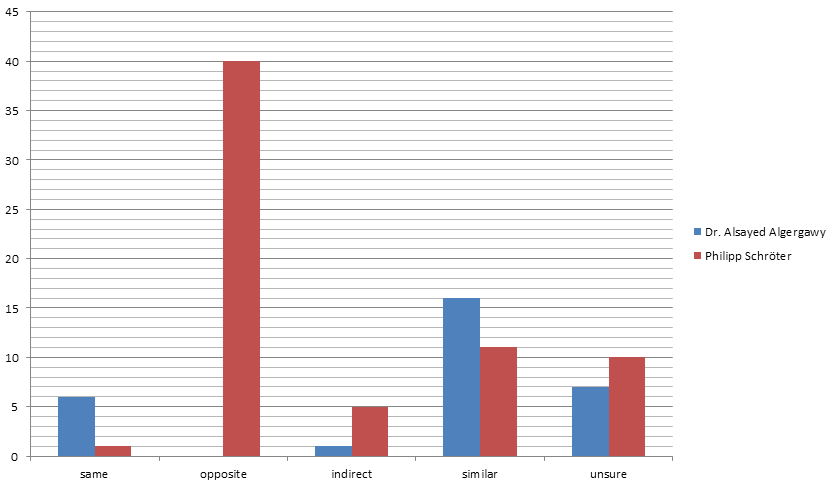
\includegraphics[width=1.0\textwidth]{pics/Vergleich-Algergawy-Schroeter_2016-11-22.png}
		\caption{Vergleich Algergawy Schröter}
		\label{fig6}
		\end{figure}
		
		\subsubsection{Fazit und Verbesserungen des Simple Ontology Matchers}
		Als erstes wurde für die gleichen Elemente, also solche mit gleicher URI, ein
		eigener Matcher geschrieben und als Bedingung in die anderen Matcher
		aufgenommen, dass die URI nicht mehr gleich sein darf. Dadurch können diese
		trivialen Ergebnisse gezielt in die Ergebnismenge miteinbezogen oder
		ausgeschlossen werden.\\
		Für den Levenshtein Matcher ergibt sich die Verbesserung, dass die obere
		Schranke für mögliche Änderungen nicht nur ein absolutes Maximum benötigt,
		sondern eines, das an die Wortlänge angepasst ist.
		
		\subsection{Evaluation 2}
		\label{subsec:Evaluation 2}
		Anhand eines vorher festgelegten Satzes an Daten wurde der im Rahmen dieser
		Masterarbeit entwickelte Simple Ontology Matcher mit der etablierten Matching
		Software
		AgreementMakerLight\footnote{\url{https://github.com/AgreementMakerLight/AML-Jar}}(\textit{AML})
		verglichen. Dieser Vergleich dient dazu, die Matcher mittels \textit{Precision
		and recall} zu verbessern.
		
		\subsubsection{Verwendete Ontologien}
		Für den Vergleich wurden zwei Ontologien verwendet, Human und Mouse. Human
		ist beschreibt die menschliche Anatomie, Mouse die von Mäusen. Diese beiden
		wurden ausgewählt, da eine hohe Überschneidung zu erwarten ist, wobei die
		innerhalb der Ontolgien verwendeten Terminologie ähnlich sein dürfte.
		
		\subsubsection{Resultat}
		Wenn man die Gesamtheit der Ergebnisse aus beiden Matching Tools betrachtet,
		erhält man eine Gesamtmenge von 2421 potenziellen Matchings. Der Simple
		Ontology Matcher hat 980 Ergebnisse, welche nicht in denen von AML enthalten
		sind (diese werden im Anschluss noch genauer analysiert). AML hat 786
		exklusive Ergebnisse. Der verbliebene Teil von 655 Matchings wurden von beiden
		vorgeschlagen. Die vollständigen Ergebnisse sind in Appendix \ref{app:second_appendix}
		aufgeführt.
		
		\subsubsection{Korrektheit der Resultate des Simple Ontology Matchers}
		Die exklusiven Ergebnisse des Simple Ontology Matchers wurden händisch auf
		Korrektheit überprüft und in verschiedene Kategorien unterteilt. Die
		Kategorien wurden gegenüber der ersten Evaluation geändert. Die Kategorien
		indirekt und ähnlich wurden entfernt, um nur die konkret zutreffenden
		Ergebnisse einzubeziehen. Die Kategorien sind \textit{gleiches} Element,
		\textit{direkte}, \textit{keine}, \textit{unsichere} Verbindung.\\
		Gleiche Element sind nicht nur Teile der Ontologie, die das
		selbe Konzept darstellen, sondern solche, die die gleiche URI haben, also bei denen
		es sich tatsächlich um ein und dasselbe handelt. Eine direkte Verbindung liegt
		vor, wenn zwischen zwei Elemente eine eindeutige Verknüpfung vorliegt, z.B.
		Unterklasse (rdfs:subClassOf) oder Gegenteil (owl:differentFrom). Wenn
		es unklar ist, ob sich ein korrektes Matching handelt, werden die entsprechenden Paare in die
		Kategorie "`unsicher"' einsortiert. Diese Ergebnisse benötigen zusätzliche
		Betrachtung von Personen mit entsprechendem Hintergrundwissen in der Domäne.\\
		
		\begin{table}
		\centering
		\caption{Kategorisierte Ergebnisse}
		\begin{tabular}{|c|c|}\hline
		Kategorie & Anzahl Paare\\ \hline
		Gleich & 7\\ \hline
		Direkt & 887\\ \hline
		Keine & 13\\ \hline
		Unsicher & 73\\ \hline
		\end{tabular}
		\end{table}
		
		\subsubsection{Analyse und mögliche Verbesserung der Matcher}
		Wenn man die vom Simple Ontology Matcher nicht erfassten Ergebnispaare
		betrachtet, fällt als erstes auf, dass es überwiegend Paare mit
		unterschiedlicher Groß- und Kleinschreibung und mit bzw. ohne Unterstrichen
		sind.\\
		Beispiele:
		\begin{itemize}
		\item \url{http://mouse.owl#MA_0001849} (right main bronchus) und \url{http://human.owl#NCI_C33486} (Right\textunderscore Main\textunderscore Bronchus)
		\item \url{http://mouse.owl#MA_0000638} (wrist skin) und \url{http://human.owl#NCI_C52752} (Wrist\textunderscore Skin)
		\item \url{http://mouse.owl#MA_0000467} (foot digit 3) und \url{http://human.owl#NCI_C52841} (Foot\textunderscore Digit\textunderscore 3)
		\item \url{http://mouse.owl#MA_0001432} (lumbar vertebra 5) und \url{http://human.owl#NCI_C32903} (L5\textunderscore Vertebra)
		\item \url{http://mouse.owl#MA_0001106} (vagus X nerve) und \url{http://human.owl#NCI_C12812} (Vagus\textunderscore Nerve)
		\item \url{http://mouse.owl#MA_0001426} (cervical vertebra 6) und \url{http://human.owl#NCI_C32244} (C6\textunderscore Vertebra)
		\item \url{http://mouse.owl#MA_0001579} (lip skin) und \url{http://human.owl#NCI_C12291} (Skin\textunderscore of\textunderscore the\textunderscore Lip)
		\item \url{http://mouse.owl#MA_0000370} (kidney capsule) und \url{http://human.owl#NCI_C12885} (Renal\textunderscore Capsule)
		\item \url{http://mouse.owl#MA_0001320} (external naris) und \url{http://human.owl#NCI_C33178} (Nostril)
		\item \url{http://mouse.owl#MA_0000715} (venous system smooth muscle) und \url{http://human.owl#NCI_C49321} (Venous\textunderscore System\textunderscore Smooth\textunderscore Muscle\textunderscore Tissue)
		\item \url{http://mouse.owl#MA_0001735} (epididymal duct) und \url{http://human.owl#NCI_C32484} (Duct\textunderscore of\textunderscore the\textunderscore Epididymis)
		\end{itemize}
		
		
		%\item Evaluation (zumeist nur für Masterarbeiten relevant)
		%\begin{itemize}
		%	\item Jede Software muss auch getestet werden. Dieses Tests werden entweder
			% mit einem vorgegebenen Datensatz erfolgen oder aber die Evaluation erfolgt auf Basis von Experimenten. In diesem Kapitel sollte daher entweder der genutzte Datensatz oder der experimentelle Aufbau beschrieben werden.
		%\end{itemize}
		%\item Ergebnis und Diskussion
		%\begin{itemize}
		%	\item Die Ergebnisse der Anwendung werden in diesem Kapitel vorgestellt und
			% anschließend diskutiert. Wenn möglich sollte die Ergebnisse in Relation zu bestehenden Arbeiten in dem Bereich erörtert werden.
		%\end{itemize}
		
	%\end{itemize}  
%\end{itemize}